\chapter{Aufgabe D9}
Für die Umsetzung der Warnfunktion durch eine LED, die einen Druckabfall-/anstieg signalisiert, wurde eine Statemachine verwendet. Diese besteht aus insgesamt fünf Stati, vier die jeweils 0,8 bzw. 1,6s dauern und die LED ein- bzw. ausschalten und dem Off-Status.
Die Variable \glqq status"' steuert die LED. Ein Ausgeben eines Tons wurde nicht umgesetzt, da im Experiment Environment, keine Tonausgabe möglich ist. Sollte dies in zukünftigen Versionen implementiert werden, kann die Variable  \glqq status"' genauso den Ton steuern. Weitere Variablen sind ausschließlich Hilfsvariablen oder zum Testen. 

\begin{figure}[h!]
	\centering
	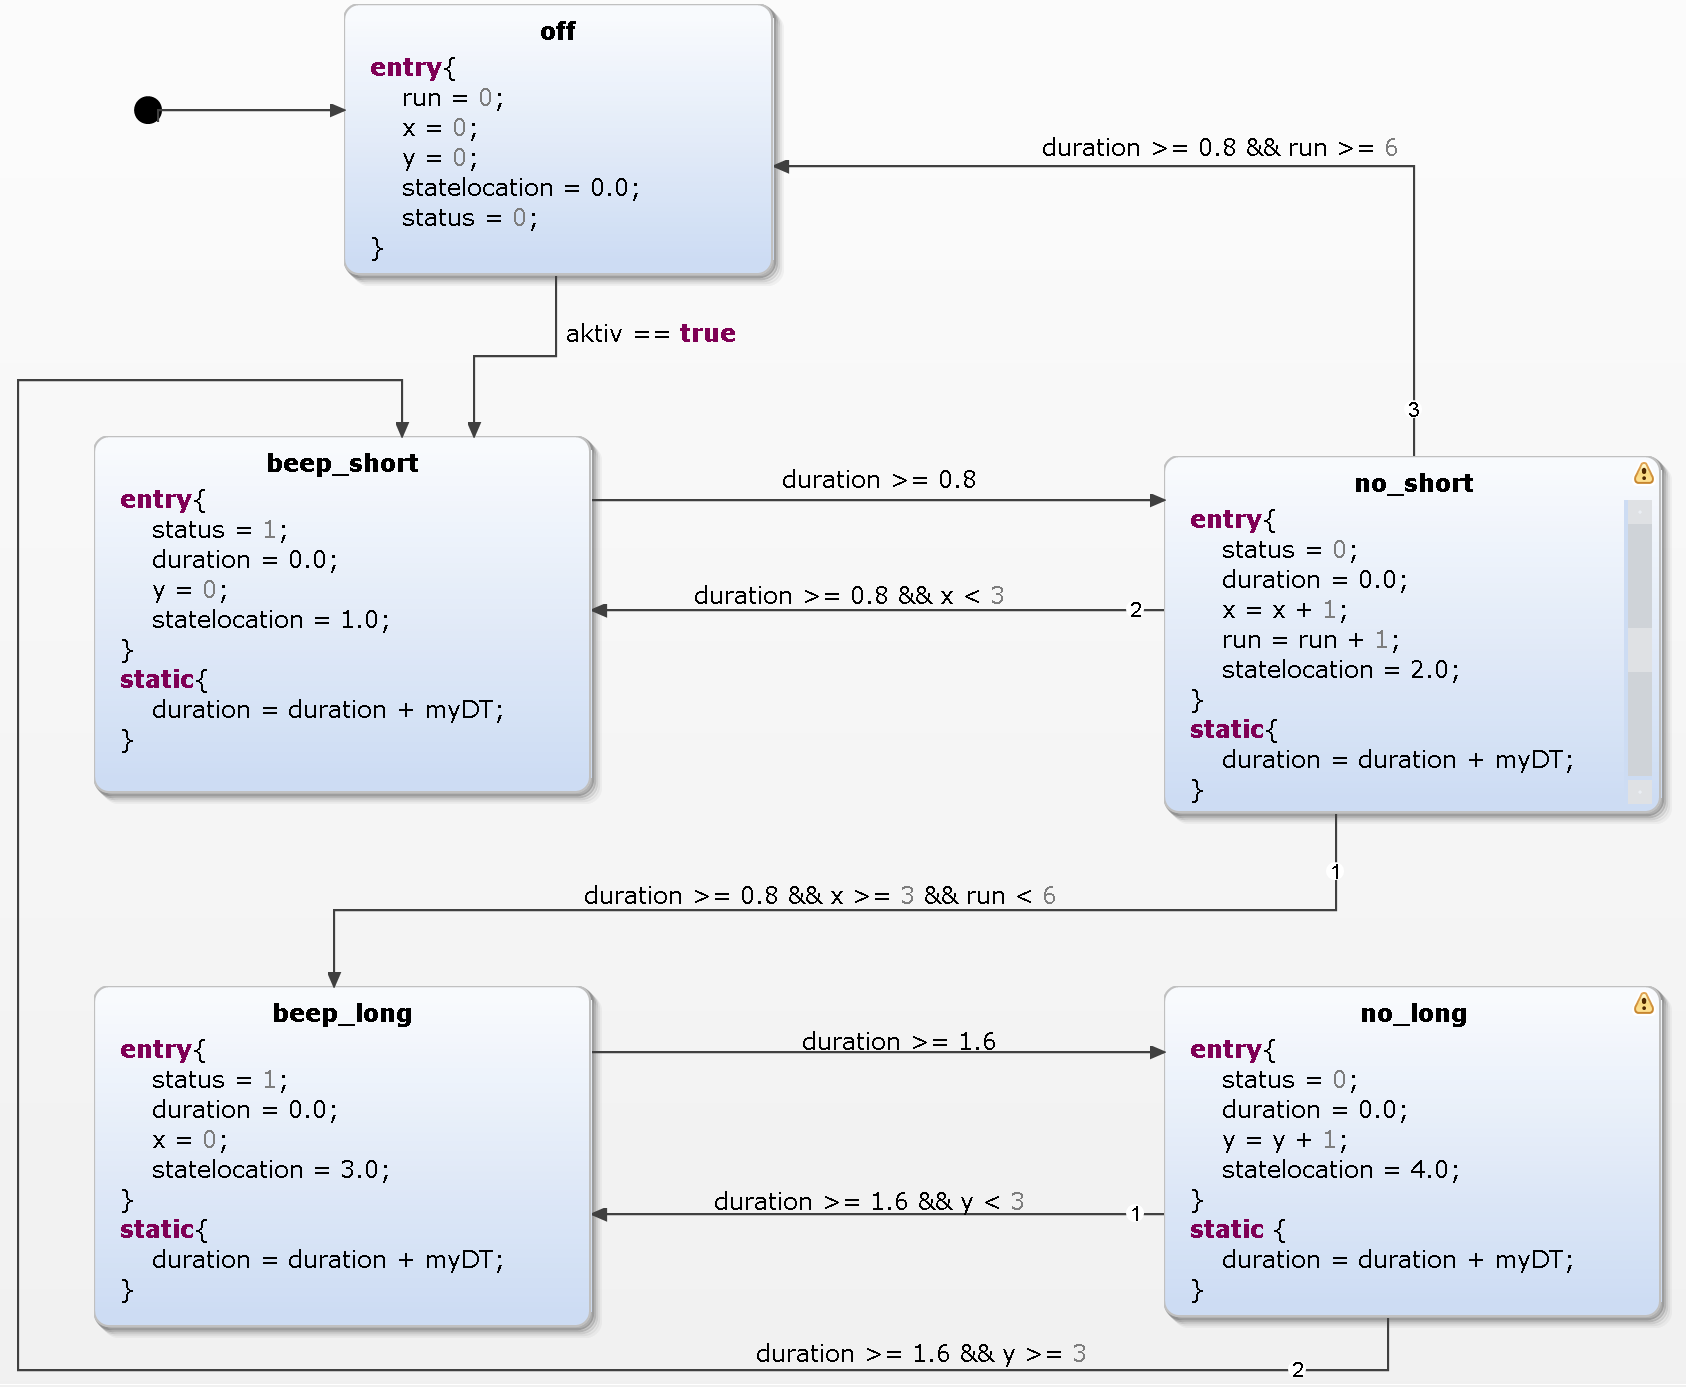
\includegraphics[width=1\linewidth]{../Graphiken/SOS_state.png}
	\caption{SOS Statemachine}
	\label{fig:SOS_state}
\end{figure}
Für die Statemachine \glqq SOS"' wurden ebenfalls Unittests durchgeführt. Zum einen wird getestet, ob die Statemachine zu jedem Zeitpunkt x im richtigen State ist. Dafür wurde eine Debugvaribale \glqq statelocation"' eingeführt.\\
Des Weiteren wird erfolgreich getestet, ob die Statemachine bei einem dauerhaften Failure aktiv bleibt.
\begin{lstlisting}
	@Test
    public void checkAllStatelocationsAndStatesActiveContinues(){}
  \end{lstlisting}
  
  
  Außerdem wird überprüft, ob die Statemachine in den Off-State wechselt, wenn nach einem vollständigem Durchlauf kein Fehler mehr vorliegt.
\begin{lstlisting}
    @Test
    public void checkAllStatelocationsActiveContinuesNot(){}
   \end{lstlisting} 
   
   
  Zuletzt wird getestet, ob die Statemachine nicht dauerhaft läuft und solange kein Fehler anliegt im Off-State verweilt.
   \begin{lstlisting}
    @Test
    public void checkAllStatesDeactiv(){}
\end{lstlisting}